\documentclass[conference]{IEEEtran}
\input epsf
\usepackage{graphicx}
\usepackage[utf8]{inputenc}
\usepackage{url}
\usepackage[nolist]{acronym}

\hyphenation{op-tical net-works semi-conduc-tor IEEEtran}
\begin{document}

\title{\LARGE BASA: Building Automation and Security on Android}

\author{
  \IEEEauthorblockN{João Miguel Marques Sampaio}\\
  \IEEEauthorblockA{Instituto Superior Técnico, Universidade de Lisboa\\ joao.mm.sampaio@tecnico.ulisboa.pt}
}


\maketitle

\begin{abstract}
Systems capable of reducing energy consumption are needed in order to reduce monetary energy costs for companies. At the same time, studies show that temperature can influence human productivity, thus simply removing \ac{HVAC} systems could impact negatively a company's employees work productivity.

Nowadays \ac{BAS} are used to manage a building, however traditional systems face a big problem, they have high monetary costs associated with installation and hardware. At the same time, the market is flooded with cheaper tablet devices with built-in sensors, connectivity and visual display.

In this document, we propose a system that utilizes an Android tablet, mounted in the room wall, running an application to achieve building automation. Our solution addresses the energy consumption problem, increases occupant comfort and offers security, including intrusion detection notification and video monitoring, to the user. The proposed system differs from traditional centralized \ac{BAS} by offering a distributed architecture with nodes deployed in every office and a user mobile application capable of interacting with the system.

\end{abstract}
% \IEEEoverridecommandlockouts
% \begin{keywords}
% Domain Registry, High availability, Load balancing, Monitoring, Registry Service, reThink H2020
% \end{keywords}

\IEEEpeerreviewmaketitle

\section{Introduction}
\label{introduction}

Buildings represent a large portion of the total energy consumed. According to the International Energy Agency, buildings represent 32\% of total final energy consumption~\cite{iea}. One way to contribute to reducing the energy consumption is to use of \ac{BAS} to improve their efficiency. Unfortunately, not all buildings are equipped with such systems. Most times, these systems offer limited functionality and can only be controlled by the building manager.

Human behavior influences the amount of energy a building requires. Depending on the occupant behavior, the building's energy cost can increase or decrease by one-third of its design performance ~\cite{ocupancy2}. Simple actions such as leaving the lighting system always on, even after the occupant has gone home, has an impact on the wasted energy used by the building. The lack of occupant detection systems in buildings prevents further energy savings, as by knowing when a room is unoccupied it is possible to shutdown unnecessary electric systems.

Nowadays, consumer smart home systems are becoming more popular. The ability to remote control the house lighting and electric devices is very appealing to consumers. At the same time smart phones and tablets flood the market at very accessible price ranges.

In this thesis, we preset a BASA (Building Automation and Security on Android) a system that uses existing Android devices to provide a \ac{BAS} capable of managing a room. Our system consists in using a wall mounted Android tablet, called Hub, to control other devices. It also allows the user's phone to interact with the Hub using a mobile application.

We designed BASA with a set of requirements in mind: The system must offer remote control of the room's lighting and \ac{HVAC} systems, allow users to automate tasks, it must be user and motion aware, it must have a affordable cost and offer good usability.

Our system is user aware and is capable of adjusting the lighting and \ac{HVAC} systems in a energy efficient way. At the same time it offers the user a \ac{IFTTT} system (trigger actions based on events) including voice recognition, for a personalized smart office experience. Finally, it provides the user with a security system. The Android camera is used to detect motion, when movement is detected and no registered person is present in the room a notification is sent to the user and a 30 second video is recorded to the cloud for latter viewing.

By using a tablet as a \ac{BAS} we are able to reduce the monetary cost of our system in comparison to traditional alternatives. The tablet offers several sensors, access to \ac{WiFi} and \ac{BT} networks, microphone, sound speaker and a touch screen. We are able to leverage the tablet sensors including illuminance, temperature and camera sensor for automation. If the tablet does not have a temperature sensor it is possible to interact with external sensors to overcome the lack of the sensor.

The below listed examples represent some automation actions possible with our \ac{IFTTT} system that contribute to decrease energy consumption and increase user comfort:

\begin{itemize}
\item If no user is present in the office then turn off the lights.
\item If user arrives at building then set temperature to 24 ºC (pre-heating). 
\item If lights are turned on and illuminance is above 120 lux then turn off the lights. (If there is  sunshine and the lights are on, we turn them off).
\item If no user is present in office and motion is detected then say "Hi! You are being recorded, smile!".
\end{itemize}

The above examples are not hard-coded into the system. They are created by the user. This ability offers great flexibility to our system to provide a personalized feel to the room.

Our system can be seen as a framework that provides a modern \ac{UI}, a \ac{IFTTT} and security system. In the future other controllable devices, triggers and actions can be added to improve the system.




\section{Background and related work}
\label{rel}

\ac{BAS} are distributed control systems capable of monitoring and controlling a multitude of individual systems in a building. Usually they are used to control a building's \ac{HVAC}, lighting, security and \ac{SAC}.
The objectives of building automation are the reduction in energy consumption, operating cost, improvement of occupant comfort, and efficient operation of building systems.



Until recently, there was no standard industry network protocol for building automation. \ac{BAS} manufacturers developed unique, proprietary communication protocols and users had to choose between many different systems. Today, we have reached a place where there are a few major platforms used for \ac{BAS} to choose from: BACnet\cite{livro_automation,bacnet:artigo1,bacnet:bib,livro_automation2}, LonWorks\cite{livro_automation2,livro_automation} and few other. 
They were designed for specialized tasks, which limits the possibilities and capabilities of every node. The automation control is usually performed on a
centralized server, commonly specified to as the Gateway. Installation may be a very complex task, requiring personalized hardware and/or software to be configured.

More recently other standards for building automation were created: ZigBee \cite{livro_zigbee} and Z-wave \cite{zwave}\cite{zigbeeAndZWave}. The new protocols vary from the previous ones by being designed to use wireless communication networks with mesh networks and allowing different manufacturers to produce products designed to to operate with these protocols. Nowadays many home automation products use ZigBee or Z-wave as their wireless communication standard allowing interoperability between products from different manufacturers.



\textbf{Modern Home Automation}

The popularity of home automation has been increasing in recent years due to higher affordability and simplicity. Home automation may include centralized control of lighting, \ac{HVAC}, appliances, security locks of gates and doors and other systems.
Vendor solutions often rely in wireless technologies to connect the various devices, thus eliminating the need to rewire the house.

Some companies like Philips have developed smart lighting products that allow remote control over the lighting system without the use of conventional light switches. The Philips hue\footnote{www2.meethue.com, last accessed on January 6$^{th}$, 2016} is a wireless lighting system. This system is quite simple, you replace existing lights with Hue light bulbs and use a device called Hue bridge to communicate with the lights using a mobile application. Both Philips hue and similar smart lights for a problem: the user cannot use a regular light switch to switch them off. By doing that the lights become disabled, the user won't be able to use the mobile application to turned them back on, requiring the user to flip the light switch back up.

One other popular product is the Nest\footnote{https://nest.com/} Learning Thermostat. It is an electronic, programmable, and self-learning \ac{WiFi} thermostat. It uses machine learning algorithm to optimize  heating and cooling of homes. Studies\cite{related:nest} show this thermostat is capable providing savings equal to about 10\%-12\% of heating usage and electric savings equal to about 15\% of cooling usage in homes with central air conditioning.

Amazon Echo\footnote{https://www.amazon.com/Amazon-Echo-Bluetooth-Speaker-with-WiFi-Alexa/dp/B00X4WHP5E, accessed 10/10/2016} is a smart speaker developed by Amazon\footnote{https://www.amazon.com/}. The device is capable of voice interaction, music playback, making to-do lists and other useful features. It can also control several smart devices using itself as a home automation hub. The main characteristic of Echo is it's voice interaction capability, any automation system would benefit by having such functionality.

Finally there are companies that provide web-based services that allows users to create simple conditional statements, which are triggered based on changes to other web. One such company is IFTTT, it allows user to trigger actions based on services such as Weather channel, Facebook, Gmail, Amazon Echo and Nest thermostat. This service allows user for example to automate their Philips Hue lights, Nest thermostat and many other services. 


There are many products for home automation in the market, in this paper we merely discussed some that contribute to our final solution. We learned smart lights have some setbacks. The Nest thermostat offers a good solution to control a \ac{HVAC} system. The only problem is it has a high monetary cost so it won't be used in our solution. Echo increases user comfort by allowing it to serve as an automation hub and allow voice interaction.We choose to implement a simple voice interaction in our final solution, as it offer many advantages. Finally we decided to implement a similar feature to the service provided by IFTTT. We allow the user to create conditional statements that trigger actions based on events in the office.


\textbf{Occupancy detection}


Human behavior influences the amount of energy a building requires. Depending on the occupant behavior, the building's energy cost can increase or decrease by one-third of its design performance \cite{ocupancy2}. 
By knowing and tracking when a room is occupied, we can provide the system with relevant information that in turn my help in taking important actions such as switching off the lights if no one is present. 

There are several different methods to determine if a person is in the room, they range from Radio Frequency Identification (RFID), Passive Infrared (PIR), Vision-based, \ac{WiFi} and Bluetooth, among other \cite{ocupancy3}.

Yuvraj Agarwal and his co-authors proposed using a mixture of PIR sensor and a simple magnetic contact switch to track when the door opens and closes, this solution provides better result in regard to a PIR only solution\cite{ocupancy1}.

Using \ac{WiFi} it is possible to estimate the number of occupants in the area. Occupants usually have mobile devices connected to the building's \ac{WiFi}, by knowing the devices currently connected to the AP it is possible to estimate their relative location. Furthermore since it does not require additional equipment, it is an economic solution.
\ac{BLE} technology is also an available solution for room user detection, leveraging the user's phone to do the detection, or asking the user to carry a \ac{BLE} beacon and have a system listening for the signals.  

A camera and image analysis software are able to identify movement between video frames. Noise detection could also provide valuable input to determine occupation, yet it is less reliable as external sounds could induce false positive occupant detection.

 


\textbf{Sensor application in Automation Systems:}
Sensors can have important contributes to \ac{BAS}, they can provide higher comfort to the occupants of the building as well as save on energy costs. Comfort can be improved using temperature sensors by regulating the building temperature to maximize occupant productivity while at the same time only spending energy when required. 

Luminosity Sensors can be used to determine if lights need to be turned on or if there is enough natural light to turn off the lights, or at the very least dim the light intensity.



\section{Architecture}
\label{act}

Nowadays it is affordable to built a device to provide \ac{BAS} functionality to a small area. This allows the room to be personalized to the occupants needs and habits.

We designed a system, named BASA, capable of controlling the lighting/\ac{HVAC} systems and offer room security. The system is described in Figure~\ref{software1} and consists of two mobile applications, one is the Hub app that runs in a tablet mounted in a wall in the room, the other is the User app that the occupant of the room can install on his personal smartphone. 


\begin{figure}[h]
\centering
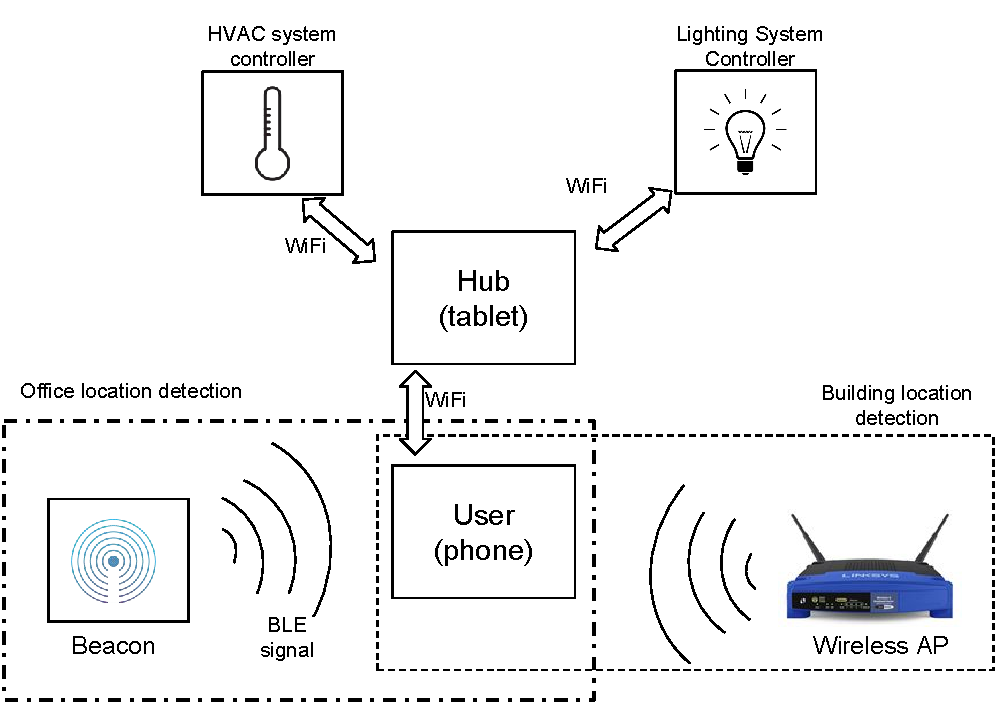
\includegraphics[width=0.5\textwidth]{Figures/harware_arch}
\caption{Overview architecture of the system}
\label{software1}
\end{figure}

\textbf{The Hub app} is responsible for controlling the \ac{HVAC} and lighting systems in the office, enforcing energy saving policies, improving occupant comfort and providing security monitoring when the user is away from the office.

The main visual features of the Hub application are: a simple \ac{GUI} to control the lights and heating/cooling system, an \ac{IFTTT} automation system that allows the user to create personalize trigger/actions rules. In the background it also provides motion detection and video recording for occasions when the user left the room but movement is detected.

\textbf{The User app} runs in the user's mobile device and offers remote control of the lighting, \ac{HVAC} and security systems provided by the Hub. Besides improving user comfort by allowing remote access to the Hub, the user app also helps the Hub with user detection, allowing the system to know when an authorized user is inside the building or room.

\subsection{Hardware Architecture}

To achieve building automation, our solution requires a tablet to act as a central control unit, a beacon device used for user detection inside the room and two other devices capable of interacting with the lighting and \ac{HVAC} systems. In Figure~\ref{hard_architecture_system} we describe the man hardware components of our system and the communication protocols used.

The tablet is where the Hub app is executed. It provides the sensors, the connectivity, the storage as well as a camera, microphone, speaker and a touch screen. 

The beacon is used for user detection, this will be explained latter in Section~\ref{architecture4}.

To control the lighting and \ac{HVAC} systems we require devices capable of interacting with existing systems that offer a way to remotely control these existing systems. These devices can be for example microcontrollers. A microcontroller allows the digital world to interact with the real world through the use of actuators that convert electric signal into mechanical actions. The microcontroller is connected to the actuators (relay) and is able to switch on/off the lights as well as controlling the HVAC. This component is needed because typically, lighting and HVAC systems do not have any type of connectivity other than the electric wires. 

\begin{figure}[h]
\centering
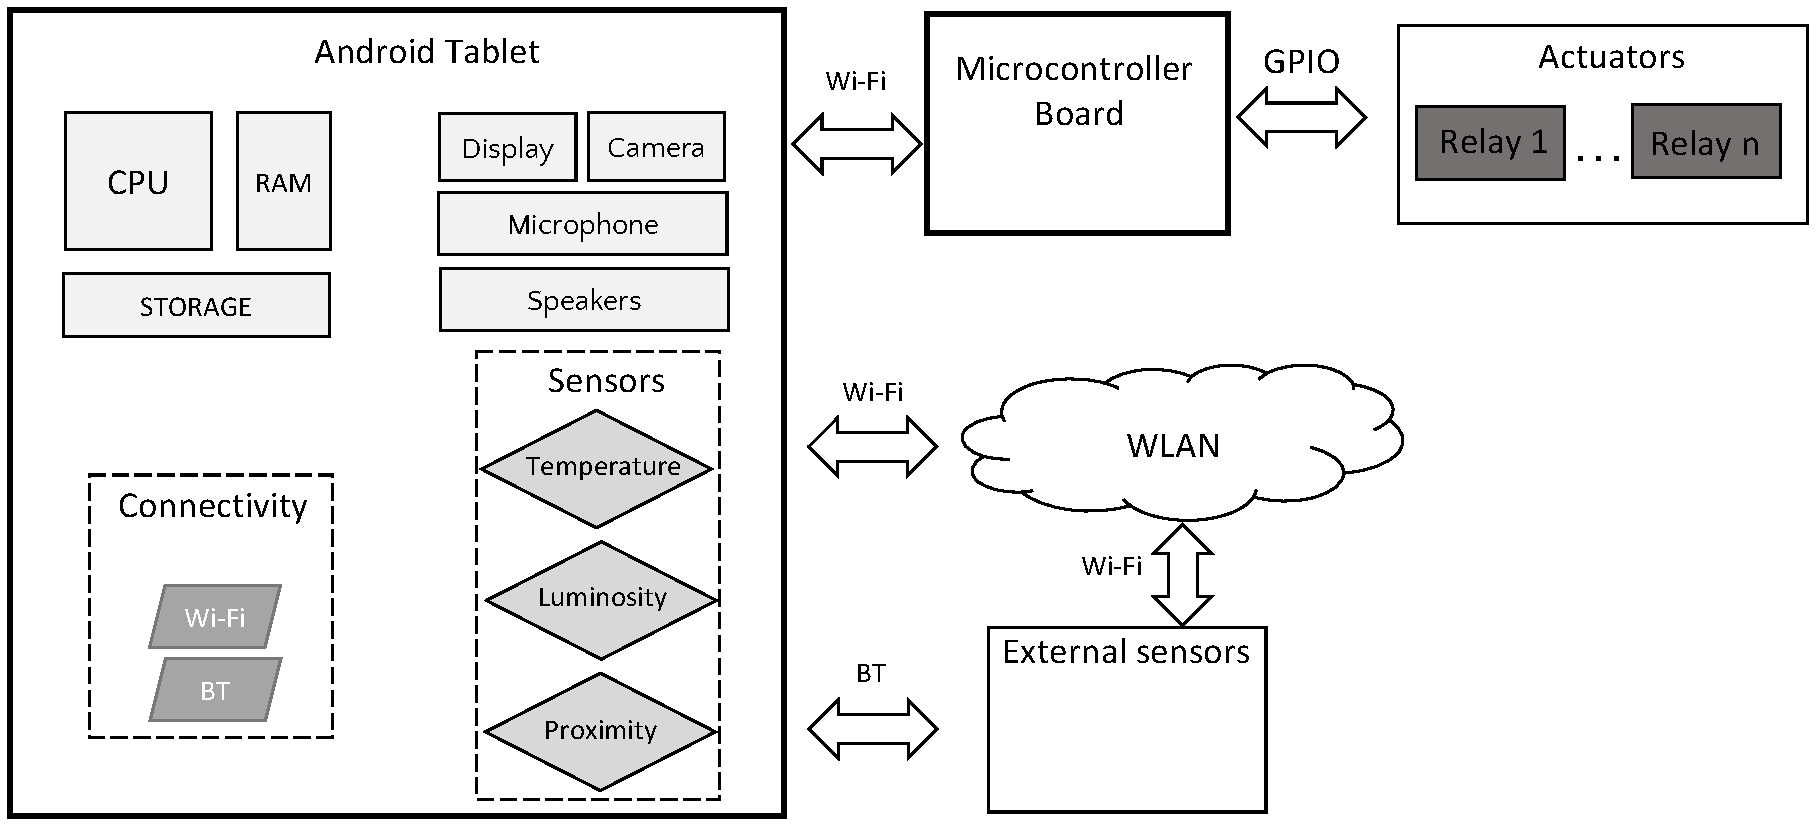
\includegraphics[width=0.5\textwidth]{Figures/arch_hardware}
\caption{Hardware architecture of the Hub}
\label{hard_architecture_system}
\end{figure}


\subsection{Software Architecture}\label{architecture4} 

In this section we present the software architecture for the mobile apps and explain some of the core functionalities of our solution.

To achieve \textbf{building automation} we propose a \ac{IFTTT} system. The user is able to create personalized chains of conditional statements, called "recipes", they are triggered based on events relevant to the office. With this system we could for example create a recipe that turns on the lights automatically when the user enters the room or shut them down when he leaves.

One of the goals of our solution is \textbf{user detection}, in order to accomplish this, we leverage two different types of location systems: \ac{WiFi} and \ac{BLE} beacon location. The location detection is handled by the user app. We use the building's \ac{WiFi} network to determine if the user is inside the building by comparing the \ac{MAC} address of available \ac{AP}s to a set of known addresses. The other location system we use is beacon location. There can be a beacon emitting \ac{BLE} signals and when this signal is detected, we know the user is near the beacon source (the office).

Regarding \textbf{office security}, we propose using the tablet's camera and analyzing the consecutive frames for changes. When no user is present in the room and a large enough number of pixels are different, we assume movement has occurred. We can then notify the user that someone is inside the room.


\subsubsection{Hub App Architecture}

We divided the Hub app into several managers, each responsible for several task. Figure~ \ref{software2}, represents the architecture of the Hub App.

\textbf{The \ac{UI}} must have a set of screens that offer:

\begin{itemize}
  \item Manual control of the lighting and HVAC systems.
  \item User registration.
  \item Creation of automation rules.
  \item Real-time ambient sensors readings.
  \item Security settings, enable/disable security monitoring and notification email.
  \item General settings, activate voice control, allow sound.
   
\end{itemize}

\textbf{Communication Layer}: The Hub app implements a web server offering an \ac{REST} \ac{API} that the user app can use to interact with. 

\textbf{The Event Manager} offers publish/subscribe service. It allows other managers to register their interest in certain events and when those happen they are notified. There can exists several different types of events: temperature reading, motion detected, user detection, etc.

The Event Manager is also responsible for the automation logic by enforcing the \ac{IFTTT} rules. The Automation Manager will check if the condition for the rule has been satisfied and trigger the action. Finally it also has a scheduler responsible for executing repetitive tasks at regular time intervals or at fixed moments.


\textbf{The User Manager} handles user registration, authentication and detection. It tracks the whereabouts of the user inside the building, in association with the User app so that, it is notified when the user enters the building or office.


\textbf{The Sensor Manager} allows access to the tablet's sensors as well as the external sensors. It abstracts external sensors into virtual sensors. It is responsible for a virtual motion detection sensor, by using the camera to detect changes that would indicate motion, as well as other data such as the opening and closing of the door.


\textbf{The Lighting Manager} is responsible for managing the lighting system. It communicates with the lightning controller (microcontroller) and synchronizes the lights state with the \ac{UI} and vice versa.

\textbf{The Temperature Manager} periodically reads the room temperature and is able to communicate with the \ac{HVAC} controller (microcontroller) to turn on/off the system when required.


\begin{figure}[h]
\centering
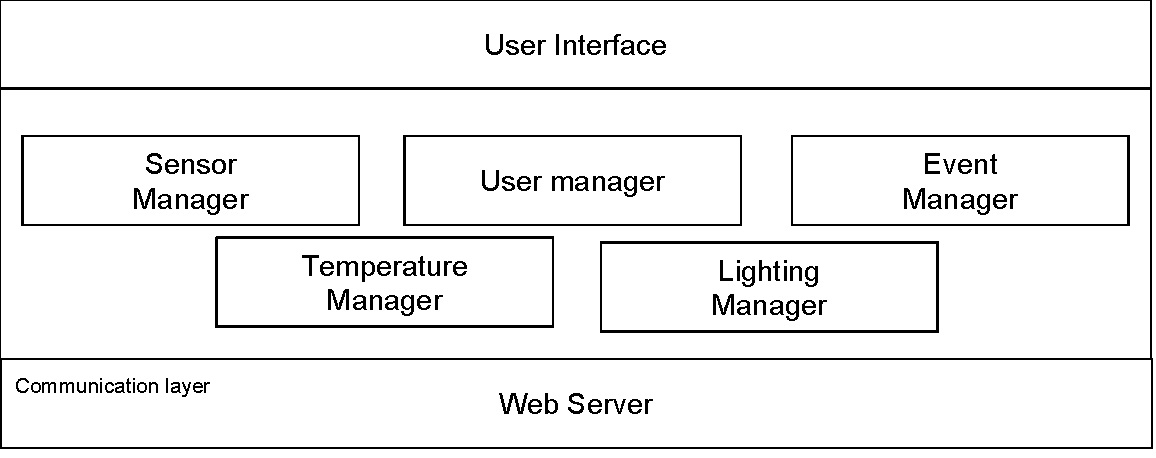
\includegraphics[width=0.9\textwidth]{Figures/software_hub}
\caption{Hub APP architecture }
\label{software2}
\end{figure}



\subsubsection{App Architecture}
The User App is simpler than the Hub App, the app is divided in \ac{UI} screens. There are no managers like the Hub architecture, the business logic is handled by each screen separately. 


The main screens are the home, lighting, temperature, security and registration screens.

Since the user app can control several Hub apps, we require a simple registration process to add the user to the Hub. We propose showing a QR-Code in the Hub registration screen, this code possesses the \ac{IP} address for the Hub and a temporary token used for registration. The user app can use the phone camera to scan the QR-Code and automatically register the user in the Hub. Then a virtual representation of the Hub is shown in the home screen.

For user detection to work when the app is not being used, we need some kind of background service to monitor the \ac{WiFi} and beacons nearby the phone. The interval between scans will be further studied in order to provide adequate time between scans and be conservative regarding the user's mobile device battery.











%
%Our main design goal is to provide reThink with a highly available architecture for one of its most important and critical components, the Domain Registry.
%We identify two actors: the \ac{CSP}, which provides and deploys the system, and the Registry Connector, a microservice also deployed by a \ac{CSP} (and part of reThink), which interacts with the Domain Registry.
%This service stores, for each Hyperty instance, the data that enables other applications to contact it.
%It provides the mapping between the identifier for each Hyperty instance (a Hyperty is used by a user in one or more devices) and the data that characterizes it.
%Therefore, the Domain Registry should provide the following functional requisites:
%
%\begin{itemize}
%\item Map identities to the Hyperty instances they are using;
%\item Provide information about a given Hyperty instance;
%\item Provide an interface for the other reThink services to harvest data.
%\end{itemize}
%
%Moreover, our system must fulfill the following non-functional requirements:
%
%\begin{itemize}
%\item \textit{Fast query response time}: Since users connect with each other through the framework reThink will provide, our service must provide low latency and a consistent performance.
%Otherwise, it could have an influence on the performance of the reThink platform;
%\item \textit{Scalability}: This service must provide a service for a large number of service providers.
%It should easily scale as needed;
%\item \textit{High availability}: Without this service, there is no way to establish a call or communication.
%Thus, our systems needs to be continuously operational.
%\item \textit{No single points of failure}: A certain amount of resilience must be provided, so that the failure of one node does not bring the others down.
%It means that at any time, any given node can be shut down or disconnected from the network while the system continues operational.
%% and the rest of the cluster will continue to operate as long as at least one of the nodes remains.
%\item \textit{Security}: Since we do not know the environment in which CSPs will deploy both the Domain Registry and the Registry Connector, will we have to ensure that the communication between these two systems can be configured in a secure manner.
%\item \textit{Developers usability}: Ensuring that every developer's computer is configured properly will delay the development process and introduce complications with software versions incompatibilities.
%Thus, from the standpoint of reThink's deployment team, the Domain Registry needs to be easily deployable will all its dependencies.
%\end{itemize}
%
%From the point of view of the \ac{CSP} that deploys the service, our design must also include a second architecture (directly linked to the first one), that enables system administration mechanisms to constantly monitor the behaviour of the deployment system, including all the interactions of its internal components.
%For that reason, the upcoming, maintainability also non-functional requirements, shall be present in our global architecture.
%
%\begin{itemize}
%\item \textit{Support for component monitoring}: Monitoring is an important part of cluster management and should be provided.
%As a result, we should be able to detect, before they lead to service outage, network component problems, as well as analyzing long-term trends (e.g. database or user base growth);
%\item \textit{Support for centralized log management}: All logs must be searchable in a single place.
%That way, we can correlate logs from different applications, which can be useful to identify user actions and applications problems.
%\end{itemize}
%
%\subsection{Core architecture}
%
%In order to comply with the functional requirements, we introduce a client-server \ac{REST} \ac{API} that exposes, and allow other systems to harvest, the services offered by the Domain Registry.
%The \ac{API} will run on application servers that will reside in the middle tier of our deployment architecture, and will return, in all cases, JSON documents containing the responses.
%This \ac{REST} service will allow the Registry Connector to register, delete and perform different types of searches on Hyperties.
%Thus, the Registry Connector will issue \ac{HTTP} requests to the Domain Registry, which, in turn, will deal with the requests and save (or retrieve) them from a persistent or in-memory database.
%Despite the knowledge that \ac{P2P} systems have an ideal system design when considering high availability and failure resilience, given the reThink project constraints for the Domain Registry, we introduce it as a client-server system, with high availability being achieved using server replication and load balancing techniques.
%Thus, as can be seen from Figure \ref{fig:first_arch}, the Registry Connector will issue \ac{HTTP} requests to the Domain Registry, which, in turn, will deal with the requests and save (or retrieve) them from a persistent or in-memory database.
%
%\begin{figure}[htb!]
%\centering
%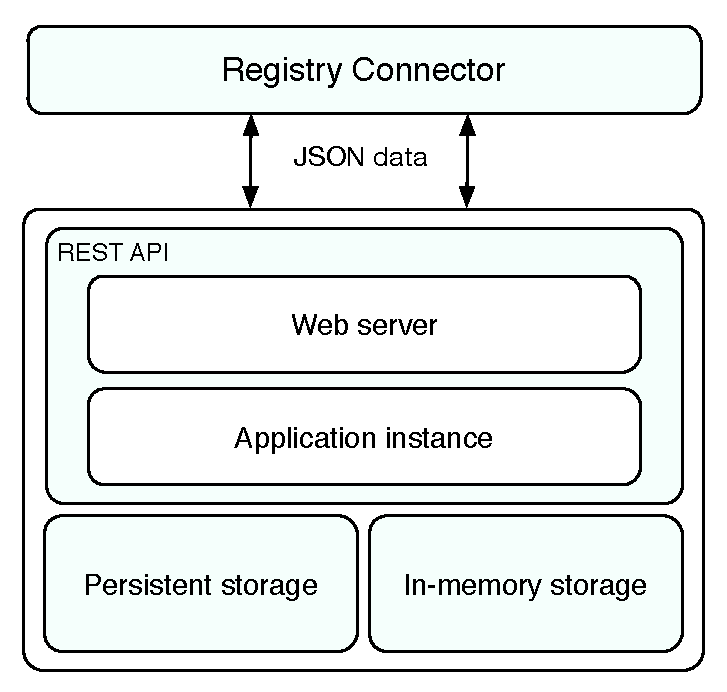
\includegraphics[width=0.25\textwidth]{functional_requirements}
%\caption{Domain Registry architecture}
%\label{fig:first_arch}
%\end{figure}
%
%Therefore, the \ac{HTTP}-based RESTful \ac{API} is defined with the following aspects: base URL, such as \url{http://api.domain.registry.com/hyperties}, standard \ac{HTTP} methods (e.g. GET, PUT, and DELETE), and a description of the state transition of the data elements.
%The \ac{API} endpoints that were defined are presented in the Table \ref{table:os}.
%The first endpoint is the most important one since it let us create, return and delete an individual Hyperty for a specific user.
%The second is used to return all the Hyperties associated to a user, and the rest of the endpoints are utilized to perform advanced searches based on Hyperties characteristics, i.e. DataSchemes and Resources.
%
%\begin{table}
%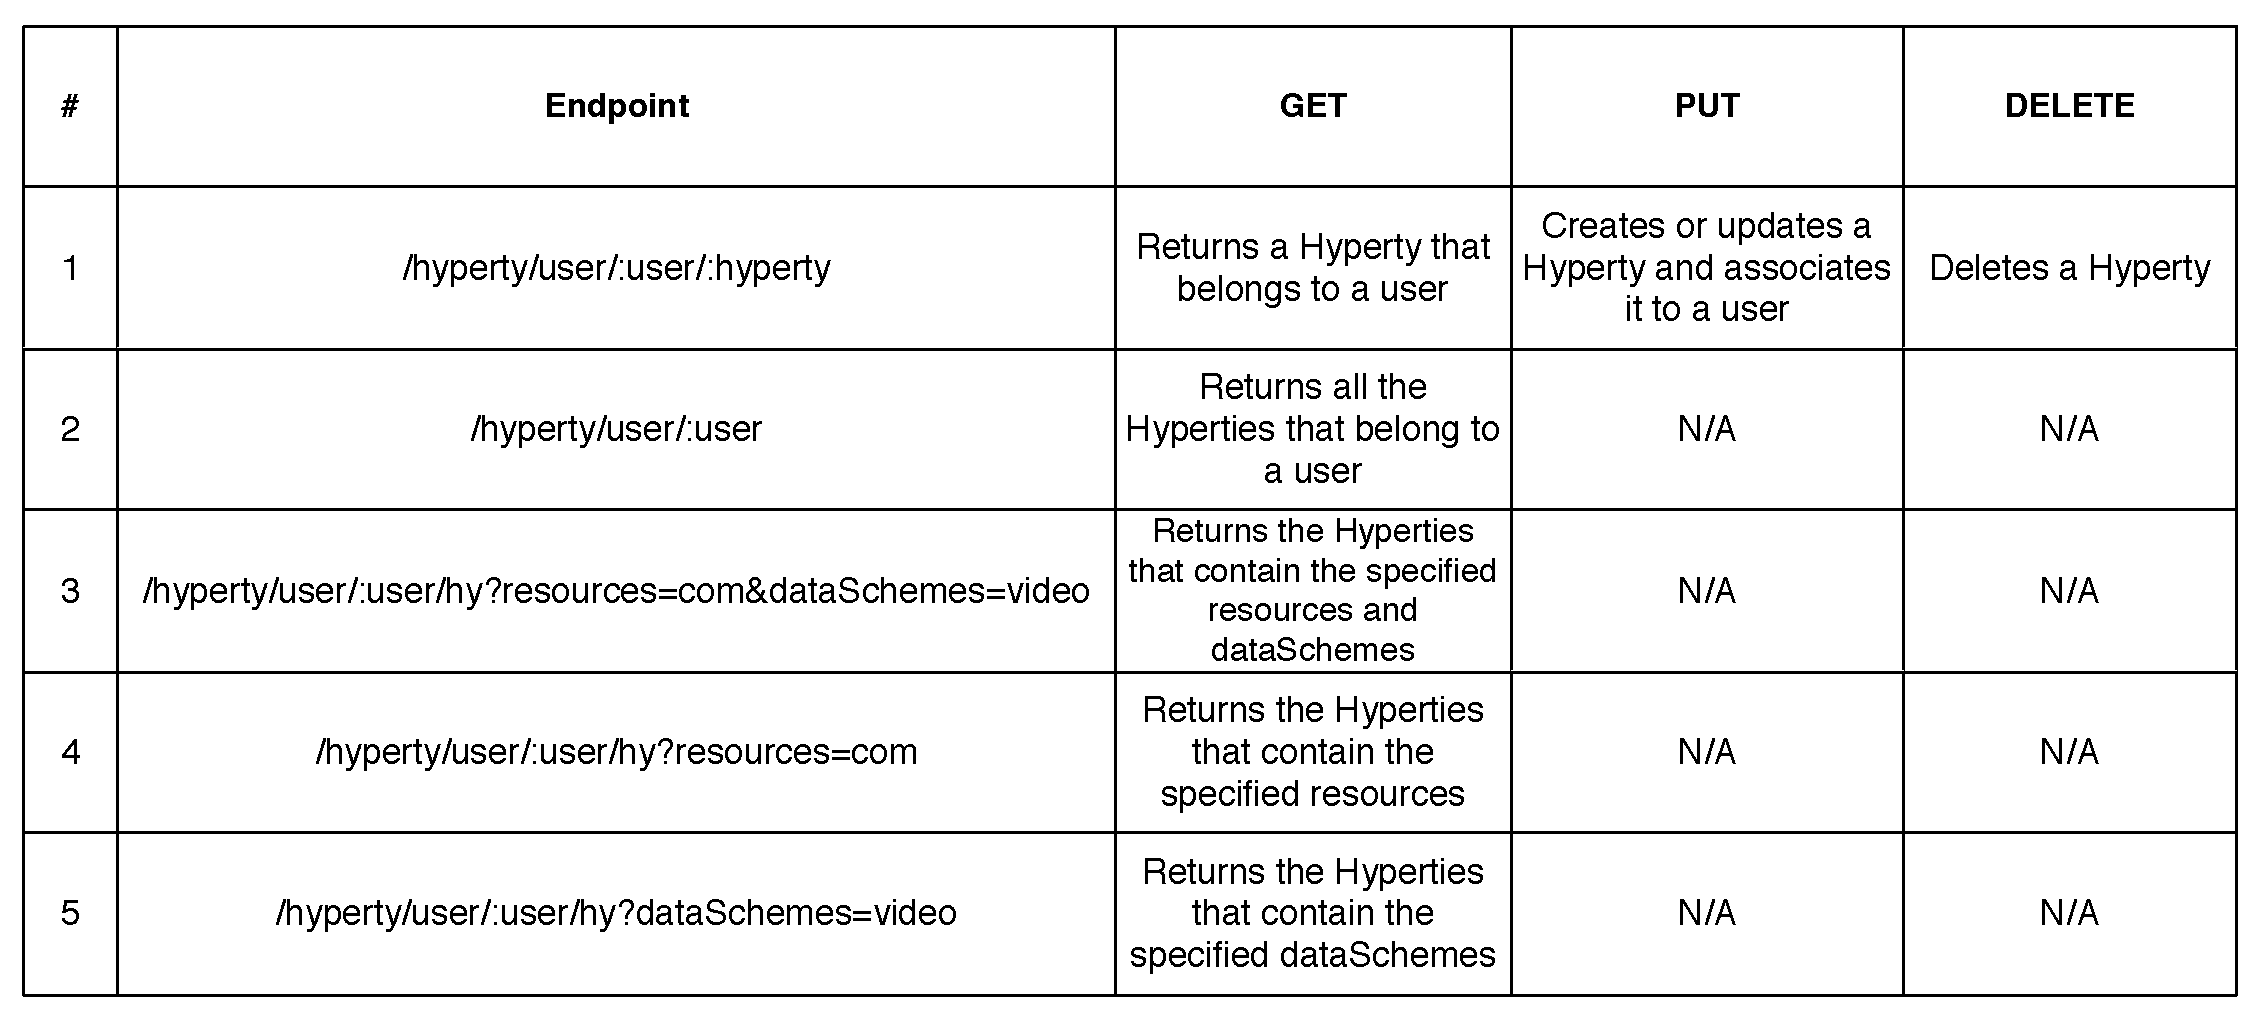
\includegraphics[width=1\linewidth]{api_table}
%\caption{Domain Registry API specification}
%\label{table:os}
%\end{table}
%
%\subsection{Deployment architecture}
%
%In the previous section we established the core architecture of the Domain Registry.
%It will be a REST API running on application servers that will allow reThink components to manage Hyperties.
%However, no non-functional requirements were addressed.
%These requirements (introduced in Section \ref{act}) are hugely important because if the Domain Registry is not reliable (for instance, while under load, or when failures happen), then it is not going to serve the client's needs. For that reason, the following topics will introduce an architecture that was designed to meet such requirements.
%
%Figure \ref{fig:app_servers_model} depicts the overall deployment architecture of the Domain Registry.
%It comprises two load balancers in failover mode, and at least, three application servers and four database nodes.
%All database nodes work in a P2P model and thus any application server can query any database server, and get the expected results.
%All application servers will run the REST \ac{API} discussed in the previous section.
%Moreover, besides this production ready architecture, and for the purposing of testing, are also available two other deployment alternatives: the first with requests being saved on memory and the second with requests being saved in a single database node.
%These two alternatives allow developers to rapidly test the \ac{API} with the purpose of getting to know, and experiment, the available endpoints.
%
%\begin{figure}[htb!]
%\centering
%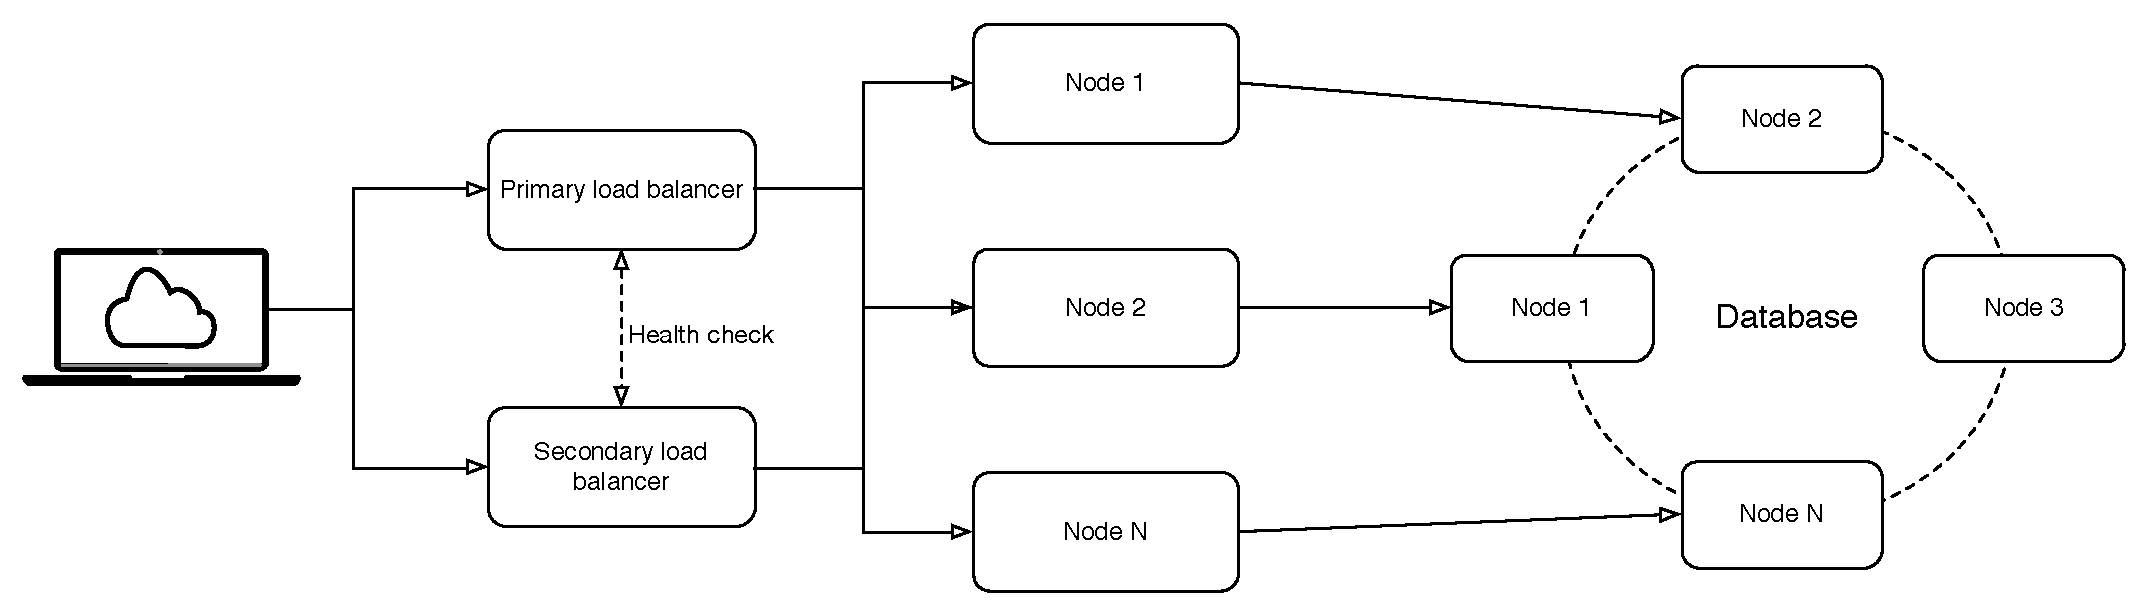
\includegraphics[width=0.49\textwidth]{arch2}
%\caption{Domain Registry main architecture}
%\label{fig:app_servers_model}
%\end{figure}
%
%Over the next sections, will be provided, individually, an explanation of each component that comprises our deployment architecture design.
%First, it is described the load balancers and floating IP mechanisms, then the database design and lastly, the security concerns that will allow a \ac{CSP} to deploy, if needed, the Domain Registry using \ac{SSL} connections.
%
%\subsection{Load balancing}
%Load balancers are added to a client server environment to improve performance and reliability by distributing client workload across multiple server machines.
%Between Layer 7 and layer 4 load balancers, we end up configuring a layer 7 load balancer because, although currently all the application servers serve the same content, as the system will grow, it may be useful to reassess the load balancing technique, and maybe employ a request awareness traffic distribution and choose different servers to deal with different requests.
%Moreover, in terms of traffic encryption, layer 4 load balancers treat connections as just a stream of information, rather than using its functions to evaluate and interpret the \ac{HTTP} requests.
%This would mean that we would be forced to configure traffic encryption on the application servers.
%Nevertheless, an architecture with a single load balancer can easily become unavailable if that load balancer fails.
%Since we needed to take into account high availability and scalability we decided to use a \ac{HA} pair of load balancers with a failover mechanism in an active/passive configuration.
%This configuration is achieved by having a floating (or virtual) IP address which can be instantly moved from one server to another in the same datacenter.
%Our infrastructure must be capable of immediately assigning this floating IP to a operational server.
%
%To achieve this goal, we used the \ac{VRRP} \cite{vrrp}, which is responsible for providing automatic assignment of an available floating IP address to participating hosts while, at the same time, ensuring that one of them is the active node (master node).
%
%While using \ac{VRRP}, failover should occur when either of the following conditions occur:
%
%\begin{itemize}
%\item \textit{When the load balancer health check on the primary server indicates that the load balancer is no longer running}: In this model, the master node constantly monitors the load balancer process, and when this process goes down, it sends a message to the slave node, which takes over almost seamlessly and instantly, allowing the service to resume.
%\item \textit{When the secondary server loses its \ac{VRRP} connection to the primary server}: If the secondary server can not reach the primary server for any reason, it will change its state to `master` and will attempt to claim the shared IP address.
%\end{itemize}
%
%In the case where there are more than one backup load balancers with the same priority values, the one with the highest IP address wins and becomes the master.
%If the primary server later recovers, it will change back to being the master node and will reclaim the shared IP address, because it will have the higher priority number in its configuration.
%
%\subsection{Database}

%Based on our requirements presented in Section \ref{act}, our infrastructure must provide high availability with no single point of failure, and every component should be easily scaled.
%Thus, our main concern while choosing a database system, is to preserve availability during network partitions and failures nodes.
%Easily scaled architectures are almost often analogous with horizontal scalability, which is the process of adding, incrementally, hardware as needed.
%Also, a database that follows this design must allow a seamless addition of new nodes with no downtimes.
%This level of scalability flexibility easily grants a very efficient deployment on either hardware components or in cloud based \ac{IaaS}.
%Our goal here, is the ability for the \ac{CSP} to scale our already developed and configured cluster as needed, and even do it on the fly (if \ac{IaaS} is used).
%Therefore, and by taking into account the above requirements, we chose to use a NoSQL database cluster with a P2P architecture, comprised of four nodes and a replication factor of three, allowing us to survive the loss of two nodes.
%As studied in Section \ref{rel}, the decentralization nature of \ac{P2P} architectures grants us the robustness needed because it removes the single point of failure from the database design.
%Moreover, with this database architecture we achieve horizontal scalability by adding more nodes as system's capacity increases.
%The overall Domain Registry capacity also increases, while the likelihood of a system failure decreases.
%
%\subsection{Security Concerns}
%Network security consists of the practices used by an organization to prevent unauthorized access or modification of networked resources.
%In our infrastructure, even though all components are to be run inside the same organization, we decided to implement a secure connection with HTTPS between the Registry Connector and the Domain Registry.
%Despite the fact that the Domain Registry interface is not available from the outside, if the \ac{CSP} decides that the connection between those two components should be secure, HTTPS can be enabled and HTTP disabled.
%This way, we give the possibility for the \acp{CSP} to choose what is the best mode to deploy the communication between such components given their infrastructure, requirements and objectives.
%However, making this connection secure introduces a significantly level of trust since, by the usage of encrypted traffic between those two components, malicious employees can not see or modify what they were not authorized to.
%
%In order to achieve this requirement, we were faced with various alternatives on how to implement \ac{TLS}/\ac{SSL} security between the client, the load balancer and the \ac{REST} application servers.
%The first scenario we studied works by having the load balancer decipher the traffic on the client side and cypher it on the server side.
%It can access the content of the request and make decisions based on that.
%Here, we have the concern off having both the load balancer and the application servers dealing with high CPU loads.
%It would probably be necessary to vertically scale these two components in order to achieve good performance levels.
%Secondly, scenario know as \ac{SSL}/\ac{TLS} offloading works by having the load balancer deciphers the traffic on the client side and sends it in clear to the backend servers.
%The application servers do not handle encrypted \ac{SSL} traffic.
%However, as in the first two scenarios, the load balancer need to be properly scaled to meet the overhead introduced by the \ac{SSL} handshakes \cite{rfc5246}.
%We end up choosing the last scenario because it is way more feasible to scale-up only one component, which in this case will be the load balancer, than to scale-up multiple backend servers.
%Also, by offloading an heavy task from the application servers, we let the servers to focus on the application itself, while at the same time we save hardware resources that can be used by the load balancers.
%Although we are focusing on application servers performance, we also know that the load balancer can itself become saturated, while dealing with \ac{SSL} connections under heavy loads of traffic.
%It is a trade-off that has to be carefully re-evaluated as the system will grew.
%
%\subsection{Operation Support Systems}
%Last but not least, we present an architecture aimed at resolving the maintainability non-functional requirement present in Section \ref{act}.
%It is system directly connected to the deployment architecture which aims at providing network management tools, i.e. monitoring and centralized logging.
%
%In Figure \ref{fig:mon_logg} is represented the overall monitoring and centralized logging architecture of our infrastructure.
%It incorporates fives servers being three of them responsible for dealing with application logs and two of them with monitoring events.
%As depicted, all three components from the deployment architecture (database servers, load balancers and application servers) generate logs and events that are then sent to other servers responsible for interpreting, parsing and displaying the results to the administrators.
%
%\begin{figure}[htb!]
%\centering
%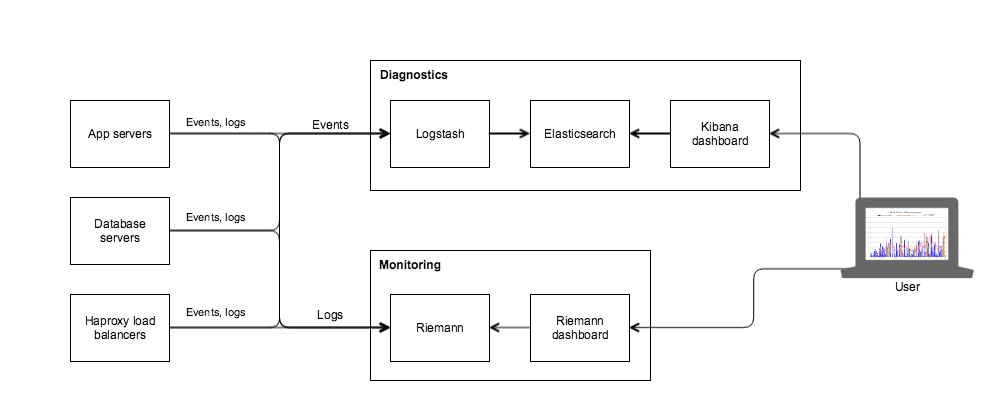
\includegraphics[width=0.51\textwidth]{L2}
%\caption{Monitoring and centralized logging.}
%\label{fig:mon_logg}
%\end{figure}
%
%\subsection{Monitoring}
%Monitoring is the process of collecting, processing, aggregating and displaying quantitative real-time events to the users.
%As we are dealing with a lot of servers, each of which with different exposed metrics and resource usage, monitoring is a crucial component of our infrastructure.
%It will help us to tell us when something is broken, or perhaps what is about to break.
%For that reason, we implemented a model where all of the servers generate and send monitoring events to another server responsible for parsing and saving them.
%We opted for a push model in which the servers responsible for dealing with the monitoring events do not do active monitoring.
%They just wait for the events to reach them, and then when they do, the servers start to perform the tasks they were assign to do.
%It is a data driven model.
%Once the deployment architecture servers realize that they have some content to be published, they will sent it without any request from the receiving end.
%This model has a big advantage over the pull based systems: the monitored nodes do not need to be constantly interrupted with demands for data that they probably do not have yet.
%Moreover, a pull based system, would mean that, as our deployment architecture grew, it would also grow the number of servers that the system would need to query.
%Therefore, a push based system was design that collect the following (most important) metrics: resource level events, requests per seconds, response codes, writes and reads and average response times.
%
%\subsection{Centralized Log Management}
%
%Gathering and parsing logs from multiple sources have several problems since most of the sources generate logs in different formats.
%Therefore, we needed a central component, which would be responsible for parsing and storing logs for future use (e.g. dashboards).
%Bearing this in mind, we deployed a system where all those logs are first received by a server responsible for normalize varying schemas and data formats.
%This normalization aims at defining a common logging format before inserting it into an analytics datastore.
%Storing is the second stage of this system.
%For displaying near real-time data to the developers, fast searches and powerful analytics capabilities were needed.
%Consequently, all of our logs are sent from the parsing server to a second one that does exactly that.
%It is vital that the chosen tool to carry out this task can be able to scale horizontally as fast as our dataset grows.

\section{Implementation}

%This section addresses the main decisions adopted regarding the implementation and configuration of the Domain Registry's internal components.
%Thus, the following sections cover the technologies that were used in the development process of those components, as well as, other modules that, although not represented in Chapter \ref{act} images, were important to perform some internal actions.
%The Domain Registry's core architecture, that is, the \ac{REST} application servers, was developed with a micro framework for creating Web applications with Java called Spark\footnote{http://sparkjava.com/}.
%Not to be confused with Apache Spark, Spark Framework, inspired by Ruby's Sinatra\footnote{www.sinatrarb.com}, is a lightweight Web framework built around Java version 8 lambda functions, which makes Spark a lot less verbose than the typically Java Web frameworks.
%This possibility started with the choice of Java as the primary programming language to develop the Domain Registry, since it was a programming language that was already being used in many reThink services.
%For code maintainability reasons it was the best choice which will allow, if needed, other developers to maintain and enhance the Domain Registry features in short periods of time.
%Regarding the executing of the Domain Registry it has two storage models: in-memory database and a persistent database.
%The persistent database is a production ready model, while the in-memory database is used for its deployment simplicity when running tests and integrations with the others components.
%The storage type is chosen \textit{a priori} with a configuration parameter.
%
%\subsection{Deployment architecture}
%For the Deployment Architecture we used several tools that will be explained throughout the next sections.
%However, and since it served as the basis of our deployment, we will introduce Docker \cite{Merkel:2014:DLL:2600239.2600241} here.
%Docker, sometimes described as lightweight Virtual Machines, is a new container technology, that eases the process of packaging and shipping distributed applications, whether on personal computers, VMs, or the cloud.
%It allows applications to be isolated within containers with instructions for what they will need to be ported from machine to machine.
%VMs allow exactly the same thing and with configuration management tools, such as Puppet, Chef or event Vagrant, the process of configuring portable and reproducible applications becomes less complicated.
%However, where Docker stands out is on resource efficiency.
%If we have fifteen Docker containers we can run all fifteen with a single command on a single VM.
%By contrast, if we have fifteen VMs, we need to boot fifteen operative systems instances with a minimum of resources from the base \ac{OS}.
%
%\subsubsection{Load balancing}
%The load balancer mechanisms implementation was split in two phases: first, its foremost role, that is, the distribution of traffic across a set of servers, and then, the failover strategy using the \ac{VRRP} protocol.
%Accordingly, the procedures introduced in this section will follow the same order.
%The most important Haproxy configuration sections are the \textit{frontend} and the \textit{backend} of the load balancer.
%The \textit{frontend} defines how requests should be forwarded to the backend servers, while in the \textit{backend} it is specified what load balance algorithm to use and which servers are available to  receive requests.
%On the \textit{frontend} we listen for incoming connections on the load balancer public IP address, add the HTTP header X-Forwarded-Proto to the end of the HTTP request, and redirect incoming traffic to the backend section.
%The X-Forwarded-Proto header defines the originating protocol of a HTTP request.
%
%On the backend of the load balancer with decided to use the \textit{roundrobin} algorithm to serve requests to the Domain Servers.
%With \textit{roundrobin}, each server is used in turn, or if some servers are more hardware powerful than the others we can assign weights to each one.
%In our setup, and since our servers are equal hardware wise, we assigned the same weight to all servers.
%
%In order for overcome a possible load balancer failure, floating IP addresses were used.
%To achieve this goal, we used a tool called \textit{keepliaved} \cite{hollenback2008improving} that implements the \ac{VRRP} protocol, allowing us to setup Haproxy nodes in a master/slave configuration.
%If the master goes down (hardware or software failure), the slave will be elected as master and will start accepting requests.
%We started its configuration by opening a \textit{vrrp\_script} on both load balancers.
%This will allow \textit{keepliaved} to monitor the Haproxy process and start recover measures when its process stops claiming a pid.
%Besides Haproxy monitoring failover, if the backup load balancer ever stops receiving \ac{VRRP} advertisements from the master, it assumes the master role and assigns the floating IP to itself.
%The only differences between the master and the slave configurations is the priority setting.
%The master server must have a high priority value than the slave.
%Otherwise, when the master node comes back up, it can not assume its role because it would have a lower priority value.
%Thus, in our configuration, the master and the slave have priority values of 101 and 100 respectively.
%\subsubsection{Database}
%We chose a NoSQL database to persistently store the data about each Hyperty instance.
%As the \ac{CAP} theorem states, it is impossible for any networked shared-data system have more than two of the three desirable properties: consistency, availability and network partition tolerance \cite{browne2009brewer}.
%Taking this into account, and since we were trying to achieve high availability with no single failures, we started the process of choosing the ideal NoSQL database.
%The ideal system would be one that was designed to be AP (from \ac{CAP} theorem), while at the same time, could provide some sort of configuration flexibility around consistency.
%We end up using Cassandra database for two reasons: it supports a multi-datacenter aware topology that can be very useful as reThink grows and second, because Cassandra's design focused on handling large write volumes.
%Regarding consistency, whenever the Registry Connector makes a read operation, it should read the last updated value.
%However, for providing strong consistency, we need to give up on availability during a network partition.
%This happens because we can not prevent disparity between two replicas that can not communicate with each other while accepting write requests on both sides of the partition.
%Consequently, we might get old data from some nodes and new data from others until it has been replicated across all devices (eventual consistency).
%However, for what we are trying to accomplish with the Domain Registry, it is preferable to have weak consistency than not having availability, since in the latter scenario communication between two reThink users will not be possible.
%Moreover, lack of availability will affect, by far, many more users than eventual consistency will.
%In essence, we designed and configured the Domain Registry Cassandra cluster to be an AP system.
%\subsubsection{Monitoring}
%The main reasons why we chose a push-based model are related to scalability as the number of machines that generate events grows.
%Riemann was designed as a distributed system monitoring tool.
%It aggregates events from network hosts and feeds them into a stream processing language so they can be manipulated and aggregated.
%We used Riemann to monitor the Domain Registry architecture because, besides it featuring a push-based model, it benefits from a stateless architecture that makes it easy to partition and distribute the load across multiple Riemann servers.
%Once again, as we are expecting the Domain Registry architecture to grow in number of servers, we are ensuring that our actual Riemann architecture can be scaled with small effort.
%
%Many quantitative data about our architecture was monitored.
%However, the only data that is processed using code written by us before being sent directly to the dashboard are event aggregator sums that represent two things: the total number of HTTP requests made to our API and the number of servers (i.e. application and database servers) that were working at a given time.
%Starting by the Haproxy load balancers, we develop a program that first, scrapped its statistics web page to a \ac{CSV} document and second, that sent the values parsed from the \ac{CSV} to our Riemann server.
%To monitor the Docker containers state, we run the \textit{docker inspect} command periodically, extract its result and sent it to Riemann for further processing.
%The API related metrics were sent to Riemann directly from the Domain Registry core architecture.
%Finally, to detect the resource level state of each machine (e.g. CPU and RAM) we used a Ruby gem called usagewatch\footnote{https://github.com/nethacker/usagewatch}, wrapped it into a script and again sent its observed values to the Riemann server.
%\subsubsection{Centralized logging}
%In order to achieve near real-time log analysis we needed text to be indexed on some sort of database.
%Text indexing refers to the technique of scanning full text documents and building a list of search terms (usually called index) \cite{salton1988term}.
%Consequently, whenever a search occurs, only the index is queried, rather than the original documents.
%For that purpose we used Elasticsearch (along with Logstash), which is a full text highly available search engine based on Apache Lucene \cite{jakarta2004apache}.
%Elasticsearch fulfills our needs by letting us perform fast searches over logs, and also by allowing horizontally scalability which is achieved by partitioning the data into smaller chunks that can be stored in several Elasticsearch  cluster nodes.
%As a means of shipping logs to Logstash, we installed in each of our servers another ELK stack underlying product called Beats\footnote{https://www.elastic.co/products/beats}.
%Beats are lightweight processes written in Golang that capture and send all sort of logs, directly or through Logstash, to Elasticsearch.
%Basically, what we did was configure each of our applications (i.e. Load balancer, REST server and database servers) to produce its logs to a predefined file which was then read by Beats and sent back to Logstash for further processing.
%Lastly, we configured Kibana.
%Kibana reads from Elasticsearch and displays its results in dashboards that can be consulted by developers.
%The overall idea of our centralized logging implementation is depicted in Figure \ref{fig:log_s}.
%
%\begin{figure}[htb!]
%\centering
%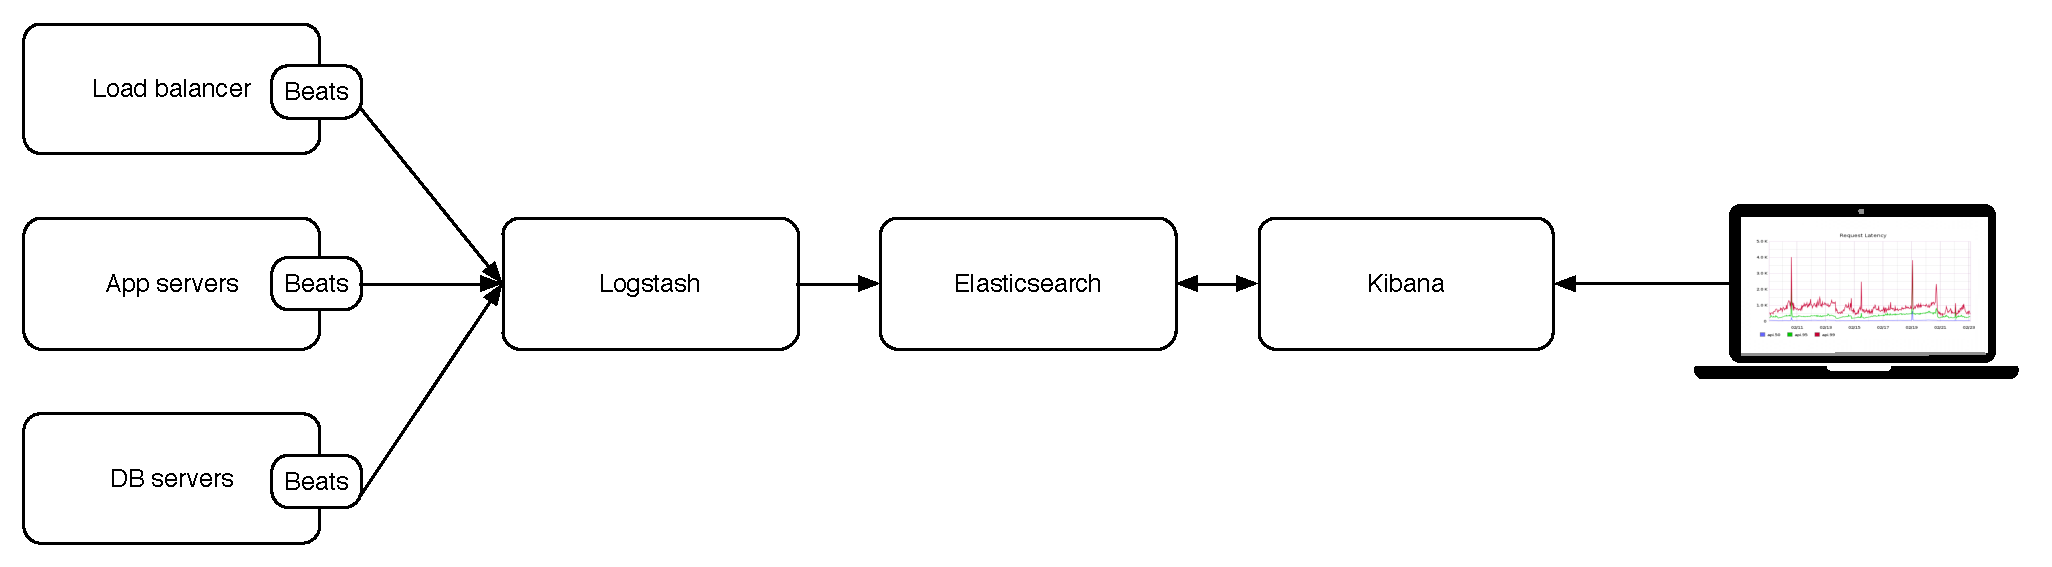
\includegraphics[width=0.5\textwidth]{loooooooooog}
%\caption{Centralized logging architecture.}
%\label{fig:log_s}
%\end{figure}

\section{Evaluation}

%In order to evaluate the developed solution, we performed several tests to measure the performance and scalability of the Domain Registry.
%Due to public cloud \ac{IaaS} costs, we did the evaluation on IST's network infrastructure using several Virtual Machines provided by DSI (\textit{Direção de Serviços de Informática}).
%Our evaluation intended to demonstrate that the Domain Registry is performant and scales horizontally while adding more nodes. Furthermore, we aim to show the responsiveness of the failover processes that were configured on the load balancers. For the first part of our tests, the following metrics were chosen to determine the suitability of the implementation:
%
%\begin{itemize}
%\item \textit{Response time for read}: As the Domain Registry is a critical component in the call establishment process, the time it takes to perform a read should be small, in the order of the tens of ms. We will test the evolution of this metric as the load on the server increases.
%\item \textit{Number of concurrent requests}: A large Service Provider is expected to have a large number of users, which will result in a high number of requests to the Domain Registry. Thus the Domain Registry should be able to scale to accommodate a large number of requests/s while providing a reasonable response time.
%\item \textit{Error rate}: Measured in number of the requests that fail to be successfully replied to within the timeout period (defined as 5s). This value should be zero.
%\end{itemize}
%
%The second part of our evaluation aimed at testing the failover processes of the Haproxy load balancers.
%For that reason, we tested the two following scenarios:
%
%\begin{itemize}
%\item \textit{Haproxy process fails}: In this scenario we purposely stop the Haproxy process to see that in fact the backup load balancer assumed the role of master load balancer;
%\item \textit{Primary load balancer fails}: Here, again on purpose, we suddenly stopped \textit{keepalived}'s process to make sure that the backup load balancer claimed the shared IP address.
%\end{itemize}
%
%The succeeding line graphs depict the first three scenarios that were evaluated.
%Each point on the graphs represents an individual test type which is the average off such test type repetitions.
%For instance, in graph from Figure \ref{fig:solicited_req_rate} the point (200,200) illustrates the first test's result in which was issued 200 requests/second and the server indeed sustained the 200 requests/second.
%The graph from Figure \ref{fig:solicited_req_rate} represents the relation between the solicited request rate and the effective request rate, with the Domain Registry infrastructure varying from one to three application servers.
%We can see that with three application servers (purple line), the Domain Registry becomes saturated at around 1750 request/second.
%After that it stabilizes on that value.
%With two application servers deployed (blue line), our prototype becomes saturated at 1200 request/seconds, and with one application server (yellow line) it saturates at around 700 requests/seconds.
%We can see that, in fact, the Domain Registry scales horizontally whenever more nodes are added.
%From Figure \ref{fig:solicited_req_rate} we observe an increase in capacity of approximately 600 requests/second when a new server is added.
%The line x=y represents the ideal scenario where the system respond successfully to all requests.
%In the following graphs we will use the effective request rate instead of the solicited request rate.
%Figure \ref{fig:average_resp_rate} presents the average response rate for an increasing request rate.
%Considering that the client and server are in the same network, a value of $\approx$ 15 ms is considered acceptable since it will not delay the reThink framework.
%In earlier tests, not represented here, with the client separated from the server, we got values below 50 ms, which is also acceptable since the two were separated by the Internet.
%As excepted, when the request rate increases past the server capacity, the server becomes saturated and the average response time increases.
%Again, each point represents the average of a single load test type.
%As an example, when we tried to perform 2000 requests/second with only one application server (blue line's last point), and as expected from the last graph, it saturated at $\approx$ 700 requests/s with an average response response delay of $\approx$ 600 ms.
%Finally, from Figure \ref{fig:errors_rate} we conclude that, although we should have no errors, when the web servers become saturated some requests are not fulfilled in less than 5 seconds.
%This value (5 seconds) was defined by us as the time we think anyone is willing to wait for a response.
%The errors we see in Figure \ref{fig:errors_rate} were not server or client errors.
%Those requests would probably be successfully if we did not set a timeout value.
%However, we can see that, until the servers become saturated there were no errors.
%
%\begin{figure}[htb]
%\centering
%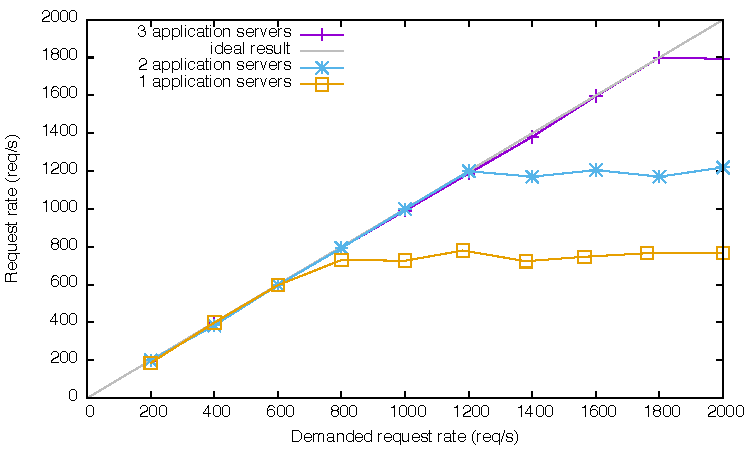
\includegraphics[width=0.35\textwidth]{demanded_request_rate}
%\caption{Demanded request rate.}
%\label{fig:solicited_req_rate}
%\end{figure}
%
%\begin{figure}[htb]
%\centering
%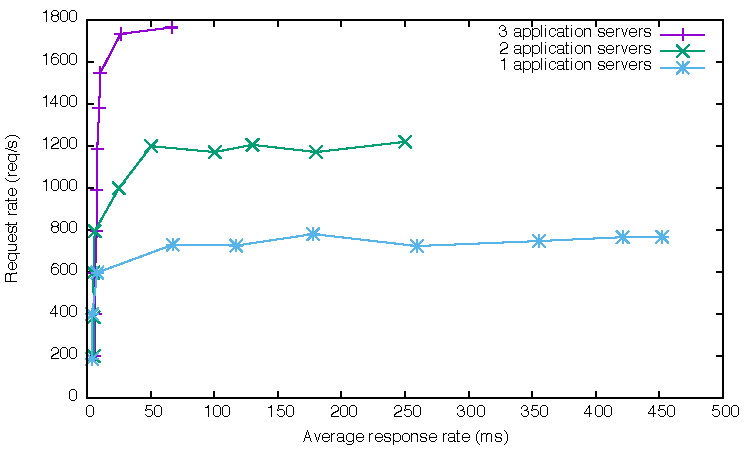
\includegraphics[width=0.35\textwidth]{avg_resp_rate}
%\caption{Average response rate.}
%\label{fig:average_resp_rate}
%\end{figure}
%
%\begin{figure}[!htb]
%\centering
%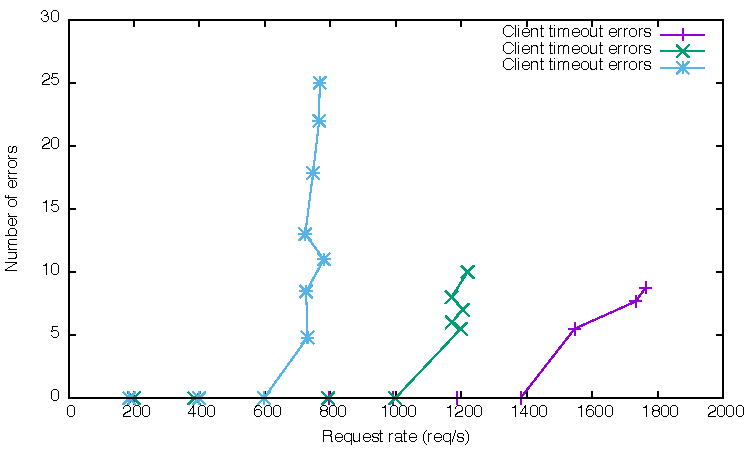
\includegraphics[width=0.35\textwidth]{errors}
%\caption{number of errors.}
%\label{fig:errors_rate}
%\end{figure}
%
%The next step was to evaluate how the Domain Registry would perform with only one database node.
%This significant drop of the cluster's size was tested because, first we get to know how the database cluster scaled, and secondly because in our deployment proposal for the reThink project partners, we presented a simple deployment with only one database node and a more complex one with four nodes.
%From both Figures \ref{fig:1_node_avg_rate} and \ref{fig:1_node_req_rate} we can see that with only one database node, the database is obviously the bottleneck of our infrastructure.
%In spite of that, the Domain Registry was able to sustain up to 1000 requests/second with average response times similar to the ones presented in Figure \ref{fig:average_resp_rate}.
%
%\begin{figure}[!htb]
%\centering
%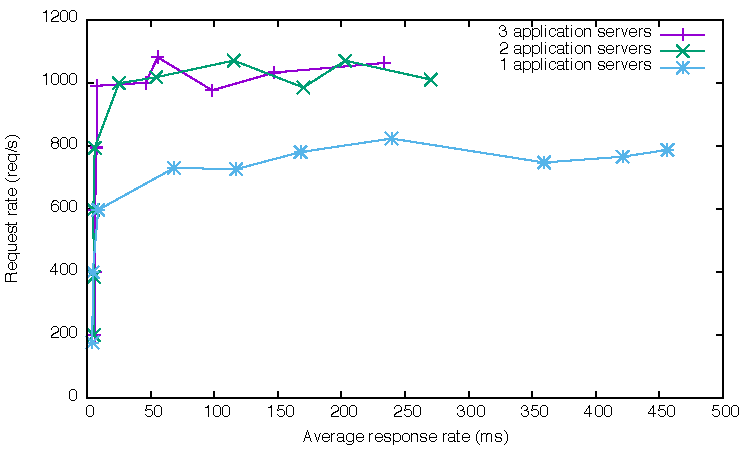
\includegraphics[width=0.35\textwidth]{1_node_avg_resp_rate}
%\caption{Average response rate with only one database node.}
%\label{fig:1_node_avg_rate}
%\end{figure}
%
%\begin{figure}[!htb]
%\centering
%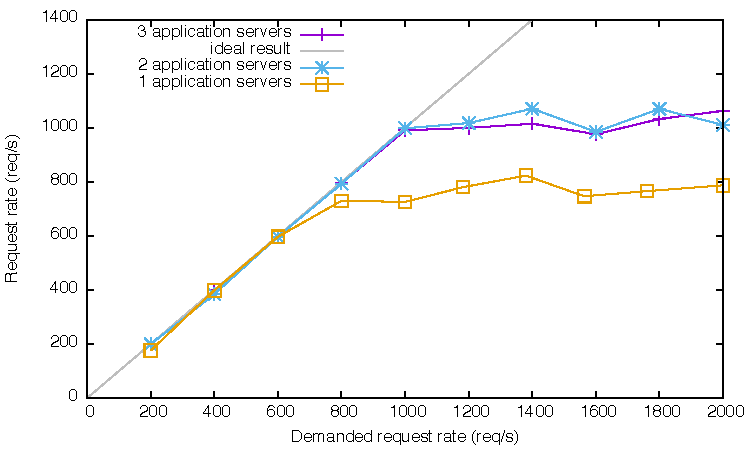
\includegraphics[width=0.35\textwidth]{1_node_demanded_request_rate}
%\caption{Solicited request rate with only one database node.}
%\label{fig:1_node_req_rate}
%\end{figure}
%
%Testing the failover mechanism of Haproxy was done using the \textit{curl} script mentioned above.
%We run the script during 60s and at $\approx$ 20 and 40 seconds we stopped first the Haproxy (Figure \ref{fig:failover_1}) and then the keepalived process (Figure \ref{fig:failover_2}) on master node.
%Regarding the load balancer fail, we set \textit{keepalived} to monitor Haproxy every 5 seconds.
%That is why there is a 5 second gap in the first graph in Figure \ref{fig:failover_1}.
%However, this value was used just for testing to actually see the transition.
%In production this value will be decreased to 2 seconds.
%That was the only value that was manually set by us.
%The other three transitions that we see on both Figure \ref{fig:failover_1} and \ref{fig:failover_2} are related to \ac{VRRP} advertisements.
%When the backup node stops receiving this advertisements it claims the shared IP address and becomes the master node (Figure \ref{fig:failover_2}).
%While assuming the master node role, if the backup node ever starts receiving \ac{VRRP} advertisements again, it elects the first node as master (because the master was set up with a higher priority level) and transits back to being the backup node, in a always listening, passive configuration (second transition of both Figure \ref{fig:failover_2} and \ref{fig:failover_1}).
%
%\begin{figure}[!htb]
%\centering
%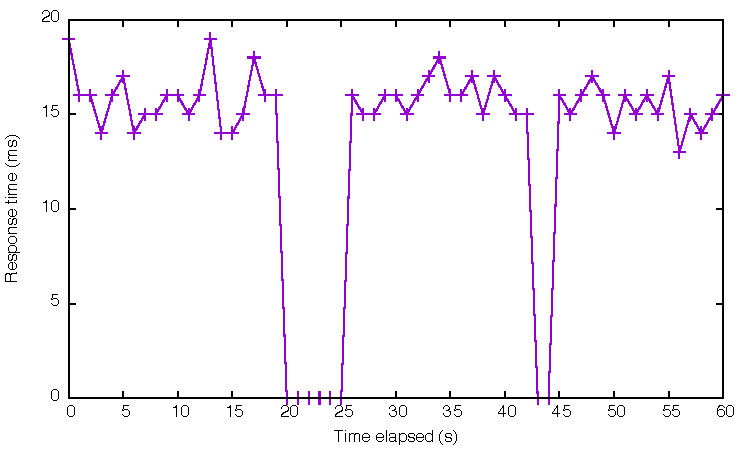
\includegraphics[width=0.35\textwidth]{keepalived_ha}
%\caption{Haproxy software failover.}
%\label{fig:failover_1}
%\end{figure}
%
%\begin{figure}[!htb]
%\centering
%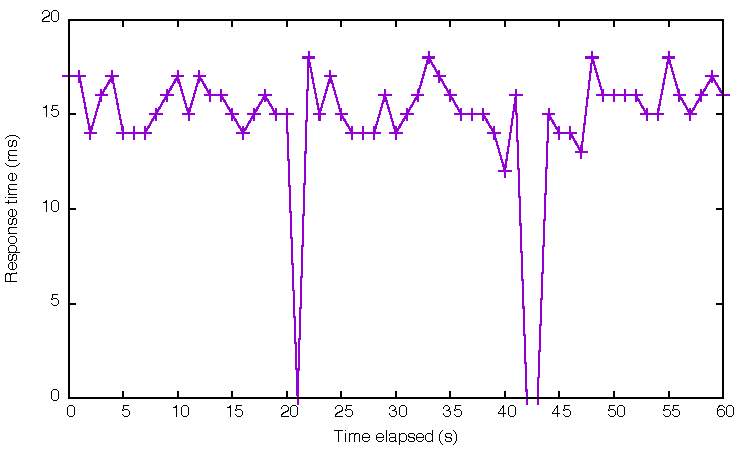
\includegraphics[width=0.35\textwidth]{keepalived_keep}
%\caption{Master node failover}
%\label{fig:failover_2}
%\end{figure}

%\subsubsection{Riemann monitoring testing}
%In order to perform the Riemann monitoring system evaluation, we used the testing tool above mentioned called Httperf solely for the purpose of visualizing changes on the dashboard and confirming that the Riemann server was receiving events.
%Figure \ref{fig:steady} shows the Riemann dashboard right after being deploying. 
%It comprises three dashboards splits, each of which comprising the resource level state of each Domain Registry server.
%At that moment it has not received any load yet.
%It shows the levels of CPU utilization, RAM and disk usage, and CPU load average for each of the servers.
%After a while we issued to load tests separated by a couple minutes.
%The first test was issued with 1000 requests/seconds and the second with 500 requests/second.
%Figure \ref{fig:riemann_load} shows the same dashboard page while the three Domain Servers were under load.
%We can see in each of the three splits that each Domain Registry server is receiving requests by analyzing the CPU usage line on the three graphs.
%Moreover, when both of the tests end, the CPU usage lines decrease to the normal state while not serving requests.
%The other lines present in the pictures did not change because those resource properties were not affected by the load tests.
%
%
%\begin{figure}[!htb]
%\centering
%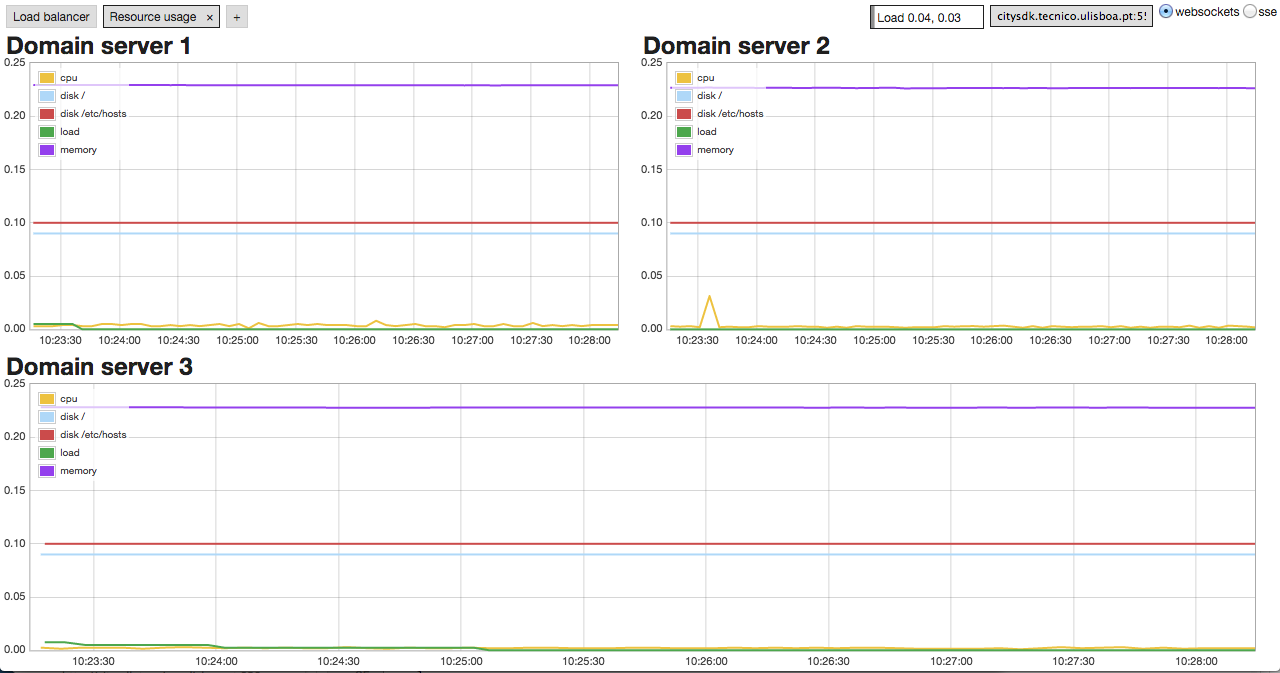
\includegraphics[width=0.5\textwidth]{resource_steady.png}
%\caption{Resource levels stable}
%\label{fig:steady}
%\end{figure}
%
%\begin{figure}[!htb]
%\centering
%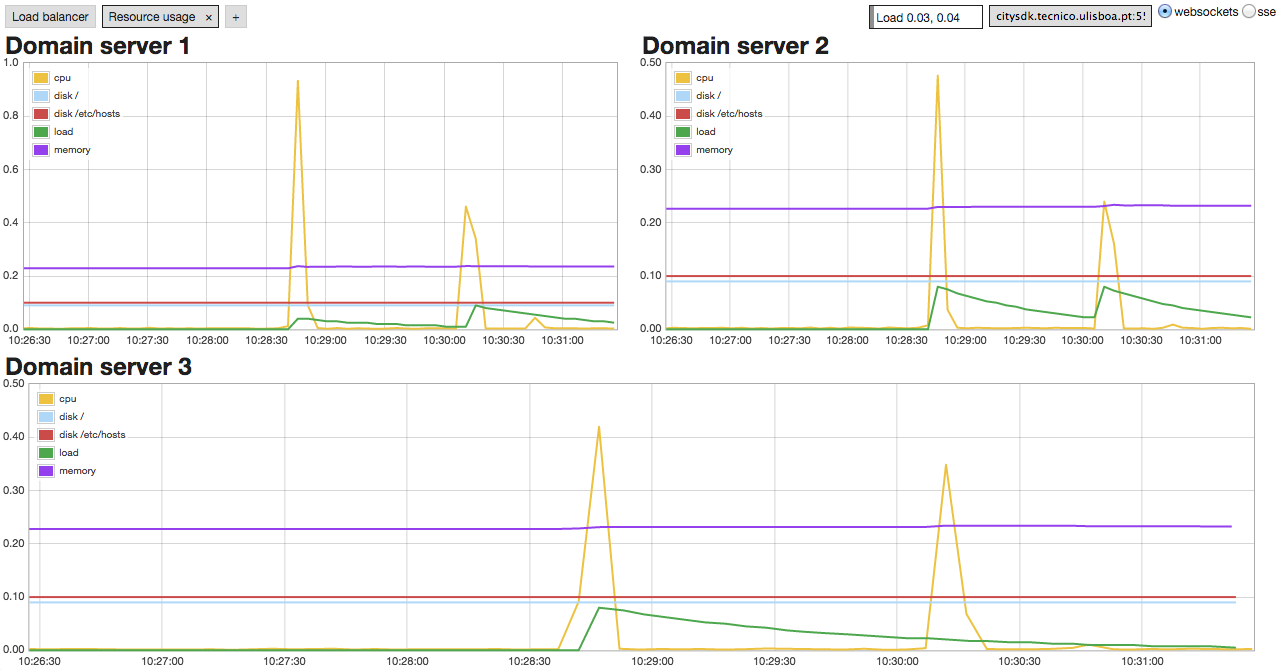
\includegraphics[width=0.5\textwidth]{resouce_under_load.png}
%\caption{Resource levels under load}
%\label{fig:riemann_load}
%\end{figure}

\section*{Conclusion}
%Our approach to develop a highly available and scalable distributed system began with an evaluation of \ac{P2P} systems and architectures.
%The idea behind a \ac{P2P} Domain Registry was each \ac{CSP} contribute to a \ac{DHT} by providing one or more nodes.
%Although being an ideal design by their scalability and fault tolerance properties, we soon understood that the major disadvantage of these kind of systems - the loss of control over where data is stored - would not work in reThink because \acp{CSP} want to control where their data is stored.
%Moreover, the existence of and the lack of full proof solutions to some security attacks, such as the Sybil \cite{douceur2002sybil} and Eclipse \cite{singh2006eclipse}, also discouraged the use of a \ac{P2P} Domain Registry.
%We then proceed to evaluate client-server systems and decided to implement the Domain Registry core architecture as a \ac{REST} \ac{API} server that would allow the creation, change and deletion of user's Hyperties.
%In order to achieve the performance requirements, we allow the Domain Registry \ac{REST} server to be replicated across several machines that will serve content in a round robin fashion, mechanism that will be performed by two load balancers in a failover state.
%Furthermore, load balancers are responsible for actively monitoring the state of each of the servers and stop sending requests to the failed ones.
%We decided to implement layer 7 load balancers which will allow us to interpret the requests in the load balancer.
%Although we are not currently using all the advantages of a layer 7 load balancer, we leave the architecture prepared for future layer 7 capabilities improvements.
%Regarding persistent data store we discussed and analysed several scalable database proposals and end up using a Cassandra database cluster that can be scaled to several nodes.
%Since we have chosen a distributed database, we matched the Domain Registry requirements with the \ac{CAP} theorem and conclude that the Domain Registry would be an AP system, that is, a high available and network partition tolerant distributed system.
%
%In order to support monitoring and centralized log management, we configured, programmed and deployed a second architecture that will interact with the first one and generate graphs and near real time information about the first architecture behaviour.
%We began to study pushing and pulling architectures, and for scalability reasons, we end up using for both logs and monitoring push-based systems in which the monitored components periodically sends events and logs for the analysis systems.
%
%We performed our evaluation on DSI's virtual machines and conclude that the Domain Registry scales horizontally when more nodes are added and that it favours response times of 15ms while serving user requests.
%In worst case scenario, that is, when a load balancer fails, we shown that the recovery process is quick, preventing the clients form using the service only a couple of seconds.
%
%Thus, we achieved the main goal that we set out at the begging of this dissertation: develop a highly available and scalable service for Hyperty reachability information with fast response times.
%
%\section{Future work}
%While we have achieved our set of goals, this work may still be improved. As the Domain Registry and its client, the Registry connector are two architectures deployed internally within a \ac{CSP}, the data generated by the Domain Registry could be serialized in another format than JSON without affecting the other reThink's components.
%JSON data favours a human readable/editable format that can be parsed without knowing any schema in advance.
%However, since the Domain Registry is not intended to be used by the rethink's end users, we propose an evaluation of the utilization of another formats, such as, Google's Protocol Buffers.
%They provide a very dense output, and thus, a very fast processing.
%However, data is internally ambiguous, and thus, requires a knowing schema to perform data decoding.
%
%Currently the Domain Registry is deployed within DSI's virtual machines.
%However, we would like to deploy the whole architecture in a \ac{IaaS} environment, such as Amazon's AWS or Google's Computer Engine, and perform a comparison analysis of the performance of both deployments.
%Moreover, related to that deployment we would like to perform a Domain Registry deployment cost analysis in such \ac{IaaS} environment.

\bibliographystyle{IEEEtran}

\addcontentsline{toc}{section}{References}
\bibliography{references.bib}

% \begin{thebibliography}{1}
%
%
% \bibitem {cantrell1}
% W. H. Cantrell, ``Tuning analysis for the high-Q class-E power
% amplifier,'' \emph{IEEE Trans. Microwave Theory \& Tech.}, vol. 48,
% no. 12, pp. 2397-2402, December 2000.
% %
%
% \end{thebibliography}

\begin{acronym}
\acro{ab}{ApacheBench}
\acro{API}{application programming interface}
\acro{AP}{Access Point}
\acro{BAS}{Building Automation Systems}
\acro{BLE}{Bluetooth Low Energy}
\acro{BSS}{Basic Service Set}
\acro{BT}{Bluetooth}
\acro{CPU}{Central processing unit}
\acro{DQPSK}{Differential Quadrature Phase Shift Keying}
\acro{FFD}{full-function device}
\acro{GFSK}{Gaussian Frequency Shift Keying}
\acro{GUI}{graphical user interface}
\acro{HTTP}{Hypertext Transfer Protocol}
\acro{HVAC}{Heating, ventilation and air conditioning}
\acro{IEEE}{Institute of Electrical and Electronics Engineers}
\acro{IFTTT}{If This Then That}
\acro{IP}{Internet Protocol}
\acro{ISM}{Scientific and Medical}
\acro{IST}{Instituto Superior Técnico}
\acro{JSON}{JavaScript Object Notation}
\acro{LAN}{Local Area Network}
\acro{LR-WPAN}{low-rate wireless personal area network}
\acro{MAC}{media access control}
\acro{MS/TP}{Master-Slave/Token-Passing}
\acro{P2P}{Peer-to-peer}
\acro{PHY}{Physical Layer}
\acro{PTP}{Point-to-Point}
\acro{PerOMAS}{Personal Office Management and Automation System}
\acro{RAM}{Random-access memory}
\acro{REST}{representational state transfer}
\acro{RFD}{reduced-function device}
\acro{ROI}{Return on investment}
\acro{SAC}{access control system}
\acro{SSDP}{Simple Service Discovery Protocol}
\acro{TCP}{Transmission Control Protocol}
\acro{UDP}{User Datagram Protocol}
\acro{UI}{User Interface}
\acro{WLAN}{wireless local area network}
\acro{WPAN}{wireless personal area network}
\acro{WiFi}{Wireless fidelity}
\end{acronym}

\end{document}
